\documentclass{beamer}

\usetheme{Boadilla}

%\includeonlyframes{current}

\usepackage{times}
\usefonttheme{structurebold}
\usepackage{listings}
\usepackage{ragged2e}

\usepackage{pgf}
\usepackage{tikz}
\usepackage{alltt}
\usepackage[normalem]{ulem}
\usetikzlibrary{arrows}
\usetikzlibrary{automata}
\usetikzlibrary{shapes}
\usepackage{amsmath,amssymb}
\usepackage{rotating}
\usepackage{ulem}
\usepackage{listings}
\usepackage{enumerate}
\usepackage{tikz}
\tikzset{
  every overlay node/.style={
    draw=black,fill=white,rounded corners,anchor=north west,
  },
}
\def\tikzoverlay{%
   \tikz[baseline,overlay]\node[every overlay node]
}%

%\setbeamercovered{dynamic}
\setbeamertemplate{footline}[page number]{}
\setbeamertemplate{navigation symbols}{}
\usefonttheme{structurebold}

\title{Software Testing, Quality Assurance \& Maintenance---Lecture 12}
\author{Patrick Lam\\University of Waterloo}
\date{January 30, 2015}

\colorlet{redshaded}{red!25!bg}
\colorlet{shaded}{black!25!bg}
\colorlet{shadedshaded}{black!10!bg}
\colorlet{blackshaded}{black!40!bg}

\colorlet{darkred}{red!80!black}
\colorlet{darkblue}{blue!80!black}
\colorlet{darkgreen}{green!80!black}

\newcommand{\rot}[1]{\rotatebox{90}{\mbox{#1}}}
\newcommand{\gray}[1]{\mbox{#1}}

\newenvironment{changemargin}[1]{% 
  \begin{list}{}{% 
    \setlength{\topsep}{0pt}% 
    \setlength{\leftmargin}{#1}% 
    \setlength{\rightmargin}{1em}
    \setlength{\listparindent}{\parindent}% 
    \setlength{\itemindent}{\parindent}% 
    \setlength{\parsep}{\parskip}% 
  }% 
  \item[]}{\end{list}}


\lstset{ %
language=C++,
basicstyle=\ttfamily,commentstyle=\scriptsize\itshape,showstringspaces=false,breaklines=true}

\begin{document}

\begin{frame}
  \titlepage
\end{frame}

\begin{frame}
  \frametitle{Last Time}
  \begin{changemargin}{2cm}
    \begin{itemize}
    \item iComment/aComment
    \item FindBugs
    \item Java Path Finder
    \item Korat
    \item Randoop
    \end{itemize}
  \end{changemargin}
\end{frame}

\begin{frame}
  \frametitle{Daikon: Dynamic Invariant Detection ([other] UW)}
  
\includegraphics[height=2em]{L11/daikon-logo}
  \begin{changemargin}{2cm}
    Goal: recover invariants from programs.\\[1em]
    Technique: run program, examine the values it computes\\[2em]
    Results:
    \begin{itemize}
    \item formal specs
    \item bugs
    \end{itemize}
    Can use Daikon on Java, C, C++, Lisp.\\[1em]
  \end{changemargin}
  \begin{center}
    \url{plse.cs.washington.edu/daikon/}\\
  \end{center}
\end{frame}
    
\begin{frame}[fragile]
  \frametitle{ESC/Java (Compaq)}
  \begin{changemargin}{2cm}
    Statically checks Java programs against specifications\\
    written in JML (Java Modelling Language).\\[1em]
    Will see more examples later. Here's one:\\
    \begin{lstlisting}[language=Java]
      //@ public invariant balance >= 0 && balance <= MAX_BALANCE;
    \end{lstlisting}
    ~\\[1em]
  \end{changemargin}
  \begin{center}
    \url{www.hpl.hp.com/downloads/crl/jtk/index.html}
  \end{center}
\end{frame}

\begin{frame}
  \frametitle{Tools you can Download}
  \begin{changemargin}{2.5cm}
    We'll survey some tools for:
    \begin{itemize}
    \item Java
    \item \alert{C/C++}
    \end{itemize}
    (or, use e.g. a programming language \\ with stronger types!)
  \end{changemargin}
\end{frame}

\begin{frame}
  \frametitle{cppcheck}
  \begin{changemargin}{2cm}
    Open-source tool that statically checks for:
    \begin{itemize}
    \item out-of-bounds errors;
    \item memory leaks;
    \item division by zero;
    \item null pointer dereferences;
    \item calls to obsolete functions;
    \item uses of uninitalized variables
    \item etc.
    \end{itemize}
  \end{changemargin}
  \begin{center}
    \url{sourceforge.net/projects/cppcheck}
  \end{center}
\end{frame}

\begin{frame}
  \frametitle{Valgrind}
  \begin{changemargin}{1.5cm}
    {\bf memcheck} is a Valgrind tool to\\ detect memory errors at runtime.\\
    Helps make your programs more correct, by finding:
    \begin{itemize}
    \item illegal reads \& writes
    \item uses of uninitialized values
    \item double frees
    \item copies with overlapping sources and destinations
    \item memory leaks
    \end{itemize}~\\[1em]
        {\bf helgrind} is a Valgrind tool to detect thread errors.\\[1em]
  \end{changemargin}
  \begin{center}
    \url{valgrind.org}
  \end{center}
\end{frame}

\begin{frame}
  \frametitle{Flawfinder}
  \begin{changemargin}{1.5cm}
    grep++: identifies non-comment calls to bad functions:
    \begin{itemize}
    \item buffer overflow risks: \\ {\tt strcpy()}, {\tt strcat()}, {\tt gets()}, {\tt sprintf()}, {\tt scanf()}
    \item format string problems: \\
      {\tt [v][f]printf()}, {\tt [v]snprintf()}, {\tt syslog()}
    \item file system race conditions:\\
      {\tt access()}, {\tt chown()}, {\tt tmpnam()}, etc.
    \end{itemize}~\\[1em]
  \end{changemargin}
  \begin{center}
    \url{www.dwheeler.com/flawfinder}
  \end{center}
\end{frame}

\begin{frame}
  \frametitle{Clang Static Analyzer (U Illinois)}
  \begin{changemargin}{1.5cm}
    (Extensible) C/C++ compiler front-end with static analyzer.\\[1em]

    The compiler: \url{clang-analyzer.llvm.org}\\[2em]
    \end{changemargin}
 \hspace*{0.5cm}    \url{clang-analyzer.llvm.org/available_checks.html}:
  \begin{changemargin}{1.5cm}
    \begin{itemize}
    \item label function arguments as ``nonnull'', \\ check for violations;
    \item the usual: memory leaks, division by 0, \\ null pointer dereferences.
    \end{itemize}
  \end{changemargin}
\end{frame}

\begin{frame}
  \frametitle{Sparse (Linux)}
  \begin{changemargin}{1.5cm}
    A ``semantic parser'' which finds faults in Linux kernel.
    \begin{itemize}
    \item mixing userspace and kernelspace pointers
    \item the usual: null pointer dereferences etc
    \end{itemize}
  \end{changemargin}
\begin{center}    
    \url{https://sparse.wiki.kernel.org/index.php/Main_Page}\\
    \url{linux.die.net/man/1/sparse}
\end{center}
\end{frame}

\begin{frame}[fragile]
  \frametitle{Splint (U Virginia)}
\hspace*{.5cm}\begin{lstlisting}[language=C]
  /*@falsewhennull@*/ bool isNonEmpty
                         (/*@null@*/ char *x) {
    return (x != NULL && *x != '\0');
  }
    \end{lstlisting}
  \begin{changemargin}{1.5cm}
    \begin{itemize}
    \item lint: the original (somewhat lame) static analyzer for C.
    \item splint: a better lint (for C, also).\\
      Checks for security vulnerabilities and coding mistakes.
    \end{itemize}
  \end{changemargin}
  \begin{center}
    \url{www.splint.org}
  \end{center}
\end{frame}

\begin{frame}[fragile]
  \frametitle{Pex (Microsoft)}
\hspace*{2cm}  White Box Unit Testing!\\
\hspace*{2cm}  \url{pexforfun.com}
\begin{center}
  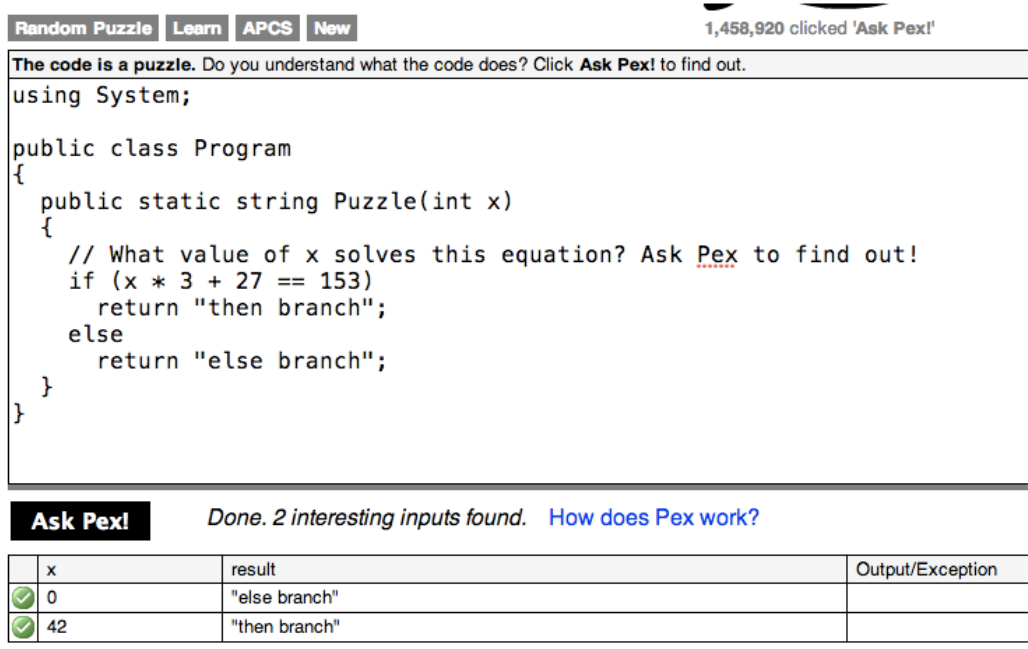
\includegraphics[width=.9\textwidth]{L11/pexforfun.png}
\end{center}
\end{frame}
      
\begin{frame}
  \frametitle{KLEE: Symbolic Execution Engine (Stanford)}
  \begin{changemargin}{2cm}
    Key idea: Use symbolic execution to automatically\\
    \hspace*{1cm} generate high-coverage test suites.\\[1em]
    Challenge: zillions of program paths, \\
    \hspace*{1cm} find the interesting ones.
    \\[2em]
    Download KLEE: \url{klee.github.io}\\
    Research paper: \\
    \url{www.doc.ic.ac.uk/~cristic/papers/klee-osdi-08.pdf}
  \end{changemargin}
\end{frame}

\begin{frame}[fragile]
  \frametitle{Symbolic Execution}
  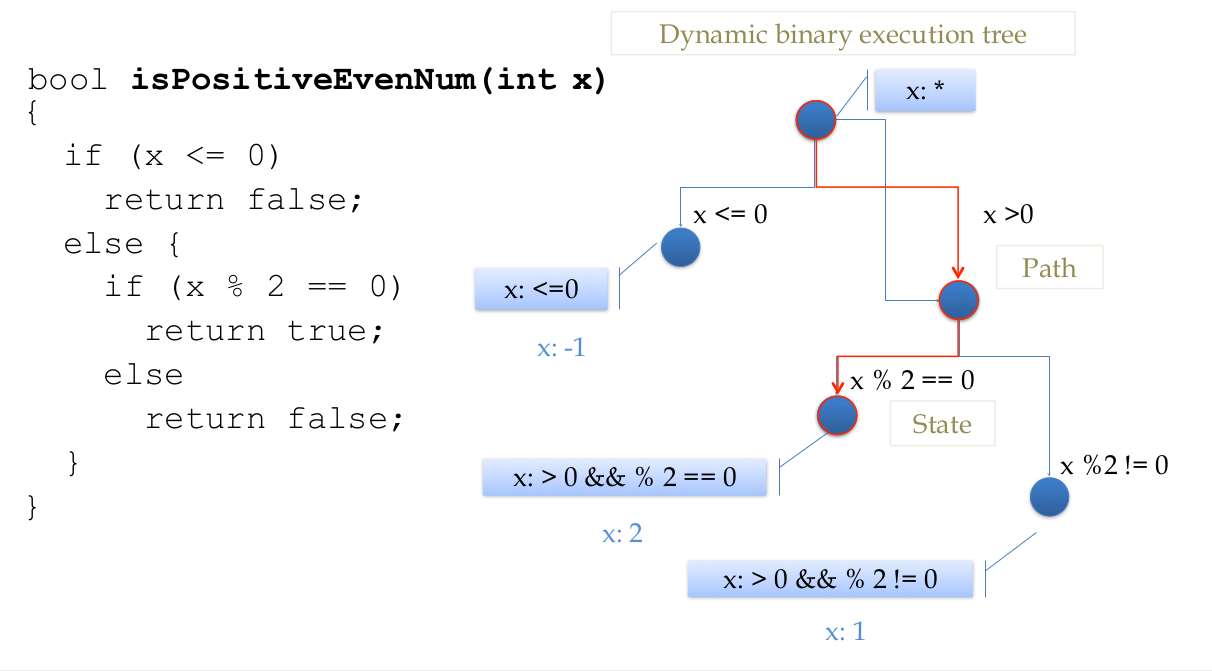
\includegraphics[width=.9\textwidth]{L11/dase.png}
  \scriptsize
  \begin{center}
  DASE: Document-Assisted Symbolic Execution for Improving Automated Software Testing.\\
  ICSE '15: Wong, Zhang, Wang, Liu, \& Tan.
  \end{center}
\end{frame}

\begin{frame}[fragile]
  \frametitle{Symbolic Execution's Problem}
  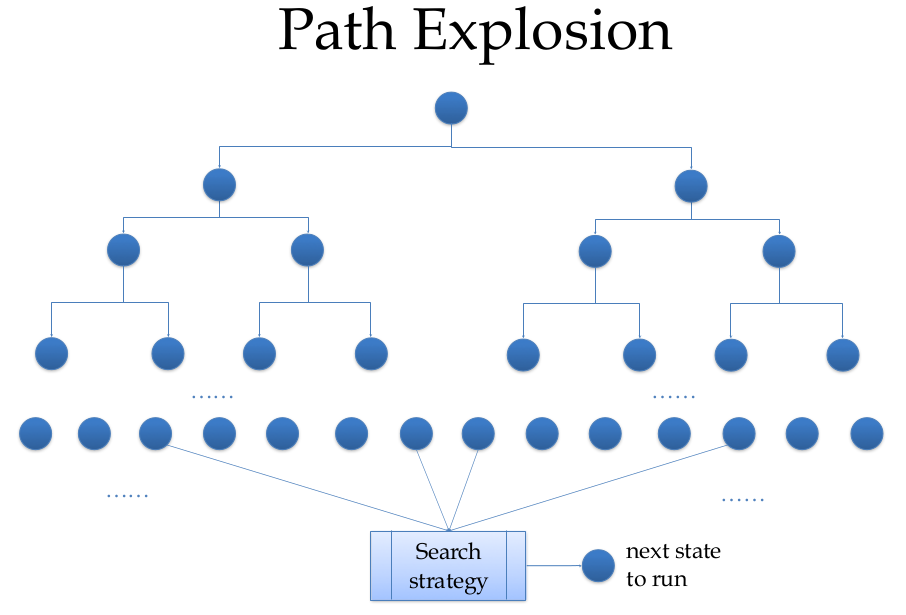
\includegraphics[width=.9\textwidth]{L11/dase2.png}
  \scriptsize
  \begin{center}
  DASE: Document-Assisted Symbolic Execution for Improving Automated Software Testing.\\
  ICSE '15: Wong, Zhang, Wang, Liu, \& Tan.
  \end{center}
\end{frame}

\begin{frame}[fragile]
  \frametitle{DASE}
  \begin{changemargin}{1.5cm}
  Use input constraints automatically extracted from documents to guide symbolic
  execution to test more effectively:\\[2em]
  DASE: Document-Assisted Symbolic Execution for Improving Automated Software Testing.\\
  ICSE '15: Edmund Wong, Lei Zhang, Song Wang, Taiyue Liu, and Lin Tan.
  \end{changemargin}
\end{frame}


\begin{frame}
  \frametitle{Defect Prediction}

  \begin{center}
    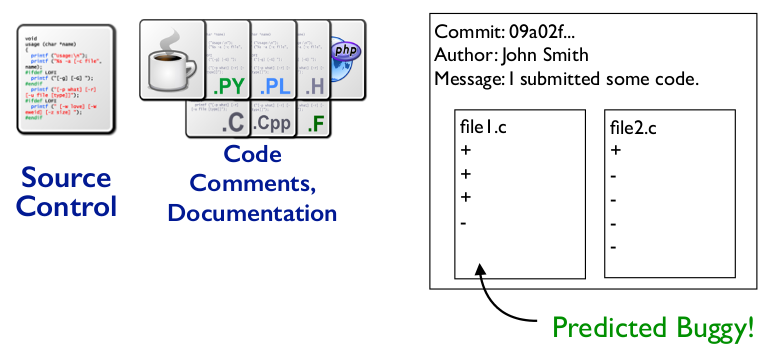
\includegraphics[width=.8\textwidth]{L11/defect-prediction}
  \end{center}

  \begin{center}
  Personalized Defect Prediction (ASE '13), Jiang, Tan and Kim.
  \end{center}
  \hfill (picture courtesy A. Hassan)
\end{frame}

\part{Other Tools from Industry}
\frame{\partpage}

\begin{frame}
  \frametitle{Coverity Static Analyzer}
  \begin{changemargin}{2cm}
    Identifies bugs in C/C++, Java, and C\# codebases.\\[1em]
    Scales to ``hundreds of users, thousands of defects, and millions of lines of code in a single analysis.''\\[1em]
    Infers must-beliefs and may-beliefs.\\[1em]
    Aims for low false positives.\\[1em]
    \url{www.coverity.com}
  \end{changemargin}
\end{frame}

\begin{frame}
  \frametitle{GrammaTech CodeSonar}
  \begin{changemargin}{2cm}
    Static analysis tool for C, C++, and Java.\\[1em]
    CodeSonar is very good at C/C++.\\[1em]
    Java bug finding performance similar to FindBugs.\\
    (CodeSonar has better user interface)\\[1em]
    Aims for high recall (find all the things!)\\[1em]
    \url{www.grammatech.com/products/codesonar}
  \end{changemargin}
\end{frame}

\begin{frame}
  \frametitle{Visual Studio (Microsoft)}

  \begin{center}
    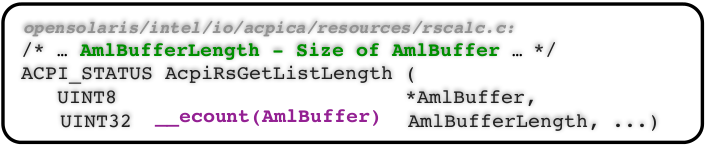
\includegraphics[width=.8\textwidth]{L11/visualstudio-sal}
  \end{center}

  \begin{changemargin}{1cm}
    Can write constraints that are related to e.g. buffer length, \\
    which are checked for bugs.
  \end{changemargin}
\end{frame}

\begin{frame}
  \frametitle{Other Commercial Tools}
  \begin{changemargin}{2cm}
    PCLint: \\ \hspace*{1em} fast, na\"ive. \url{www.gimpel.com/html/pcl.htm}\\[1em]
    PVS-Studio: \url{www.viva64.com/en/b/0149}\\[1em]
    Fortify: helps find security vulnerabilities \\
    \hspace*{1em} in a wide variety of languages + config files\\[1em]
    Intel Parallel Studio XE: \\ \hspace*{1em} Static Security Analysis for C++, Fortran\\[1em]
    Klocwork Insight: \\ \hspace*{1em} finds security issues \& bugs in C/C++, Java, C\#
  \end{changemargin}
\end{frame}

\begin{frame}
  \frametitle{Tools, more for Development}
  \begin{changemargin}{2cm}
    ScalaTest: flexible testing framework for Scala\\[1em]
    ScalaCheck: random test generators, \\
    \hspace*{2em}property-based testing\\[1em]
    Jacoco: code coverage \\
    \hspace*{2em} (many others also, eg EclEmma)\\[1em]
    Atlassian Bamboo: continuous integration server
  \end{changemargin}
  \hfill \scriptsize suggested by Michael Viana
\end{frame}

\begin{frame}
  \frametitle{Homework}
  \begin{changemargin}{2cm}
    Draw a decision tree to help a software tester/developer select an appropriate tool (if any) for a given project.\\[1em]
    \begin{itemize}
    \item more than one tool may be appropriate.
    \end{itemize}
    ~\\[1em]
    Pick two tools, use them, and compare them.
  \end{changemargin}
\end{frame}
    
\end{document}
